% !TeX spellcheck = it_IT
\section{Reflection in Java}

% Slide 03

La \textbf{Java Core Reflection API} fornisce una API piccola, type safe e sicura per quanto riguarda l'introspection per classi e oggetti nella JVM.

In generale, ci sono un po' di limitazioni su cosa permette la reflection (policy, moduli di sicurezza nelle nuove versioni), non è mai stato un focus primario per Java, ma è sempre stata utilizzata.

Se permesso dalla security policy, la API può essere usata per:
\begin{itemize}
	\item Costruire nuove istanze di classe e nuovi array

	\item Accedere e modificare campi di oggetti e classi

	\item Invocare metodi

	\item Accedere e modificare elementi di un array
\end{itemize}
Intercessione su classi e oggetti è proibita.

Ci sono applicazioni della suite Java che fanno uso delle reflection, come:
\begin{itemize}
	\item Documentazione automatica (javadoc, \dots)

	\item Tool per IDE: browser, inspectors, debuggers; molti sono scritti in Java e fanno uso della reflection

	\item Serializzazione/deserializzazione: costruire una rappresentazione binaria per backup o trasmissione, ricreare un oggetto a partire dalla sua forma serializzata

	\item RMI Remote Method Invocation: i dati usati per chiamare metodi da remoto di fatto vengono serializzati per chiamare dall'altro lato il metodo vero
\end{itemize}

%s4
%Story time: cosa è stato aggiunto nelle varie versioni

Nelle varie versioni di Java le classi e interfacce disponibili per la reflection sono cambiate, da Java 13 in avanti le classi e interfacce coinvolte sono:
\begin{itemize}
	\item \texttt{java.lang.Object}, superclasse di ogni classe in Java, tutto è \texttt{Object}

	\item \texttt{java.lang.Class}, classe che rappresenta le classi e le interfacce di Java come oggetti, ogni oggetto "porta con sé" la propria \texttt{Class} (da un oggetto \texttt{p}, \texttt{p.getClass()} permette di ottenere un oggetto \texttt{Class} che descrive la struttura di \texttt{p})
\end{itemize}
In breve, \texttt{Object} è la base di tutti gli oggetti runtime, mentre \texttt{Class} è la base di tutti i meta-oggetti ("descrive" gli oggetti).

\subsection{\texttt{java.lang.reflect}}

La libreria \texttt{java.lang.reflect} contiene
\begin{itemize}
	\item \texttt{java.lang.reflect.Member}, interfaccia comune a campi, metodi e costruttori. Permette di sapere cose come nome (\texttt{getName()}), classe dichiarativa (\texttt{getDeclaringClass()}) e i modificatori (\texttt{getModifiers()}, ad esempio \texttt{public}, \texttt{private}, \dots)

	\item \texttt{java.lang.reflect.AccessibleObject}, permette di controllare l'accessibilità di un membro (\texttt{isAccessible()} restituisce se l'oggetto è accessibile tramite reflection), ma anche di modificarla (\texttt{setAccessible(boolean flag)}). Si tratta della classe base per
	\begin{itemize}
		\item \texttt{java.lang.reflect.Field}, rappresenta un attributo di una classe, permette di agire su un campo, permette di leggere e agire su tipo, nome e modificatori del campo. Ad esempio, \texttt{getName()}, \texttt{getType()} e \texttt{getModifiers()} permettono di sapere tipo, nome e modificatori del campo, mentre \texttt{get(Object obj)} e \texttt{set(Object obj, Object value)} permettono di accedere al valore del campo

		\item \texttt{java.lang.reflect.Method}, rappresenta un metodo, permette di leggerne le informazioni (\texttt{getName()}, \texttt{getReturnType()}, \texttt{getParameterTypes()}, \texttt{getModifiers()}, \dots) ed eventualmente invocarlo dinamicamente su un'istanza o sulla classe stessa se è \texttt{static}

		\item \texttt{java.lang.reflect.Constructor}, rappresenta un costruttore dichiarato in una classe, permette di ottenere informazioni sul costruttore stesso (\texttt{getName()}, \texttt{getParameterTypes()}, \texttt{getModifiers()}, \dots), ma anche di istanziare nuovi oggetti
	\end{itemize}

	\item \texttt{java.lang.reflect.Proxy}, permette di creare oggetti Proxy dinamici, ovvero un oggetto che implementa una o più interfacce specificate e intercetta tutte le chiamate ai loro metodi, che vengono inviate a un \texttt{InvocationHandler}

	\item \texttt{java.lang.reflect.InvocationHandler}, interfaccia che gestisce le invocazioni dei metodi sui proxy dinamici, ha un solo metodo astratto \texttt{invoke(Object proxy, Method method, Object[] args) throws Throwable}. Permette di modificare la logica prima o dopo l'invocazione del metodo, o anche modificare l'esecuzione a seconda delle condizioni, senza andare a toccare il metodo concreto
\end{itemize}

Si hanno anche
\begin{itemize}
	\item \texttt{java.lang.annotation.Annotation}, interfaccia radice per tutte le annotazioni in Java, permettendo anche reflection sulle annotazioni

	\item \texttt{java.lang.instrument.Instrumentation}, interfaccia che permette di intercettare e modificare bytecode delle classi durante il caricamento nella JVM
\end{itemize}

%s5
In Java, il modello di reflection è quello a \textbf{meta-oggetti}, anche se solo predefiniti, ovvero ci sono meta-oggetti generici per il ruolo del campo, per il ruolo di Metodo, \dots

%s6
Limiti della reflection in Java:
\begin{itemize}
	\item Il MOP non è causalmente connesso: togliendo l'intercessione non c'è rischio di modifica e conseguenti inconsistenze all'interno del bytecode Java; viene considerata un rischio

	\item \texttt{Class} è dichiarata come \texttt{final}, non possono essere create nuove meta-classi

	\item Non ci sono operazioni MOP per modificare le classi, quindi non si può facilmente creare e modularizzare trasformazioni da classe a classe
\end{itemize}

Le class-to-class transformation esistono, ma sono usate dagli sviluppatori della stdlib, non da chi programma in Java (\texttt{Cloneable}, \texttt{Remote}, \texttt{Serializable}, sono trasformazioni class-to-class, ma un programmatore Java non può crearne di altre).

\subsubsection{\texttt{Object}}

\texttt{Object} definisce metodi alla quale rispondono tutti gli oggetti, "radice" della gerarchia, metodi di default che si potrebbero volere in una classe.
\begin{minted}{java}
class Object {
    public final Class<?> getClass() { ... }
    protected Object clone() { ... }
    public boolean equals(Object obj) { ... }
    public int hashCode() { ... }
    public String toString() { ... }
    public final void notify() { ... }
    public final void notifyAll() { ... }
    public final void wait() { ... }
    ...
}
\end{minted}

Non rilevante per fare reflection.

\subsubsection{\texttt{Class}}
%s9
La classe \texttt{Class} mette a disposizione gli elementi principali per qualsiasi attività riflessiva.
\begin{minted}{java}
public final class Class<T> extends Object {
    public static Class<?> forName(String className) { ... }
    public static Class<?> forName(Module module, String name)
        { ... }
    // from Java 22
    public static Class<?> forPrimitiveName
        (String primitiveName) { ... }

    public T newInstance() { ... } /* deprecated since 9 */
    public boolean isInstance(Object obj) { ... }

    public String getName() { ... }
    public Class<? super T> getSuperclass() { ... }
    public Module getModule() { ... }
    public Class<?>[] getInterfaces() { ... }

    public Class<?>[] getDeclaredClasses() { ... }
    public Method[] getDeclaredMethods() { ... }
    public Annotation[] getAnnotation() { ... }
    public Constructor<?>[] getConstructors() { ... }
    public Field[] getFields() { ... }

    public boolean isAnnotation() { ... }
    public boolean isArray() { ... }
    public boolean isEnum() { ... }
    public boolean isRecord() { ... }
    ...
}
\end{minted}

\newpage

Esempio di metodo per tornare il nome di una classe in maniera stampabile:
\begin{minted}{java}
class MOP {
    public static String classNameToString(Class<?> cls) {
        if (!cls.isArray()) return cls.getName();
        return cls.getComponentType().getName() + "[]";
    }
}
\end{minted}
Torna il nome della classe sotto forma di stringa, gestendo correttamente gli array.

Esempio di uso:
\begin{minted}{c}
jshell> MOP.classNameToString(String.class)
$2 ==> "java.lang.String"

jshell> var a = new Integer[]{1, 2, 3}
a ==> Integer[3] {1, 2, 3}

jshell> a.getClass()
$4 ==> class [Ljava.lang.Integer;

jshell> MOP.classNameToString(a.getClass())
$5 ==> "java.lang.Integer[]"
\end{minted}

Altro esempio, metodo per tornare tutta la gerarchia al di sopra di una classe:
\begin{minted}{java}
import java.util.ArrayList;
import java.util.List;
class MOP {
    public static Class<?>[] getAllSuperClasses(Class<?> cls) {
        List<Class<?>> result = new ArrayList<Class<?>>();
        for (Class<?> x = cls; x != null; x = x.getSuperclass())
            result.add(x);
        return result.toArray(new Class<?>[0]);
    }
}
\end{minted}
Mette in un array tutte le super-classi trovate, ogni volta andando a quella sopra tramite un loop, quando la successiva è \texttt{null}, siamo arrivati a \texttt{Object} e non c'è niente sopra.

Esempio di uso:
\begin{minted}{c}
jshell> MOP.getAllSuperClasses(java.util.ArrayList.class)
$4 ==> Class[4] {
    class java.util.ArrayList, class java.util.AbstractList,
    class java.util.AbstractCollection, class java.lang.Object
}
\end{minted}

Metodi a disposizione di \texttt{Class<T>}:
\begin{center}
    \resizebox{\textwidth}{!}{%
        \ttfamily
        \begin{tabular}{l l l}
            \normalfont \textbf{Member Access} & \normalfont \textbf{Class Properties} & \normalfont \textbf{Context Access} \\[6pt]

            getAnnotations()        & getComponentType()      & getClassLoader() \\
            getAnnotation()         & getDeclaringClass()     & getInterfaces() \\
            getClasses()            & getEnclosingClass()     & getModule() \\
            getConstructors()       & getEnclosingConstructor()& getPackage() \\
            getConstructor()        & getEnclosingMethod()    & getProtectionDomain() \\
            getDeclaredAnnotations()& getEnumConstants()      & getResourceAsStream() \\
            getDeclaredAnnotation() & getModifiers()          & getResource() \\
            getDeclaredClasses()    & getName()               & getSigners() \\
            getDeclaredConstructors()& getRecodComponents()   & \\
            getDeclaredConstructor()& getSuperClass()         & \\
            getDeclaredFields()     & isAnnotationPresent()   & \\
            getDeclaredField()      & isAnnotation()          & \\
            getDeclaredMethods()    & isAnonymousClass()      & \\
            getDeclaredMethod()     & isArray()               & \\
            getFields()             & isAssignableFrom()      & \\
            getField()              & isEnum()                & \\
            getMethods()            & isHidden()              & \\
            getMethod()             & isInterface()           & \\
            & isPrimitive()           & \\
    \end{tabular}}
\end{center}

Nella prima categoria sono presenti 3 "tipi" di metodi:
\begin{itemize}
    \item Senza la \texttt{s} finale (al singolare, ad esempio \texttt{getField(String name)}), restituisce uno specifico membro identificato dal nome (parametro)

    \item Con la \texttt{s} finale, restituisce un array con tutti i membri accessibili

    \item Con \texttt{Declared}, restituisce tutti e soli gli elementi dichiarati all'interno della classe, pubblici o privati, ma non ereditati
\end{itemize}

La seconda categoria permette l'introspezione sulle proprietà della classe stessa, informazioni sulla natura della classe stessa, ad esempio \texttt{getName()} restituisce il nome completo della classe.

L'ultima categoria fa riferimento all'accesso, permette di ottenere informazioni riguardo il contesto di runtime all'interno del quale la classe esiste, ad esempio \texttt{getClassLoader()} restituisce il ClassLoader che ha caricato quella classe.

\subsubsection{\texttt{Method}}
%s13?
La classe \texttt{java.lang.reflect.Method} permette di fare introspezione sui metodi.
\begin{minted}{java}
public final class Method extends Executable
            implements AnnotatedElement, Member {
    public Class<?> getReturnType() { ... }
    public int getParameterCount() { ... }
    // Inherited by Executable
    public Parameter[] getParameters() { ... }
    public Class<?>[] getParameterTypes() { ... }
    public Class<?>[] getExceptionTypes() { ... }
    public Object invoke(Object obj, Object... args)
        throws IllegalAccessException, IllegalArgumentException,
        InvocationTargetException { ... }
    ...
}
\end{minted}

Il metodo \texttt{invoke} permette di eseguire dinamicamente un metodo su un oggetto, gestendo boxing e unboxing automatico tra primitivi e wrapper e restituisce il risultato come \texttt{Object}

\subsubsection{\texttt{Parameter}}

La classe \texttt{java.lang.reflect.Parameter} rappresenta ciascun singolo parametro formale di un metodo o costruttore, permettendo di ottenere tutte le caratteristiche di ciascun parametro.
\begin{minted}{java}
public final class Parameter implements AnnotatedElement {
    public Set<AccessFlag> accessFlags() { ... }
    public String getName() { ... }
    public Class<?> getType() { ... }
    public boolean isVarArgs() { ... }
    ...
}
\end{minted}
Un oggetto \texttt{Parameter} non si crea direttamente, lo si ottiene tramite \texttt{getParameters()}. I metodi al suo interno permettono di agire sui parametri ottenuti.

Si ha un problema con l'uguaglianza: \texttt{invoke} chiede solo \texttt{Object}, quindi effettua un boxing dei parametri, questo potrebbe causare problemi nel momento in cui i valori sono confrontati tramite \texttt{==}, in quanto confronta il riferimento all'oggetto e non il valore stesso, due oggetti \texttt{Integer} diversi risulteranno sempre diversi, anche se contengono lo stesso valore (in realtà se è un intero fino a 255 esistono dei singleton per gestire lo specifico caso, da 256 potresti avere problemi).

Esempio di due metodi per restituire i parametri di un \texttt{Method}
\begin{minted}{java}
class MOP {
    public static String parametersToString(Method m) {
        var mt = Arrays.asList(m.getParameterTypes());
        return IntStream.range(0, m.getParameterCount()).boxed()
            .map(i -> {
                return MOP.classNameToString(mt.get(i))
                    + " p" + (i + 1);
            }).collect(Collectors.joining(", "));
    }
    public static String formalParametersToString(Method m) {
        return Arrays.stream(m.getParameters())
            .map(p -> MOP.classNameToString(p.getType())
                + " " + p.getName())
            .collect(Collectors.joining(", "));
    }
}
\end{minted}

Il primo metodo restituisce i parametri di un \texttt{Method} dato, fornendo un nome arbitrario (\texttt{p1}, \texttt{p2}, \dots), in quanto \texttt{getParameterTypes()} non fornisce il nome del parametro. Il secondo metodo usa \texttt{getParameters()}, che restituisce anche i nomi dei parametri, quindi si possono usare i nomi definiti all'interno del sistema al posto di quelli arbitrari.

Esempio di metodo per tornare la firma di un altro metodo
\begin{minted}{java}
import java.lang.reflect.Method;
import java.util.Arrays;
import java.util.stream.Collectors;
import java.util.stream.IntStream;
class MOP {
    public static String headerToString(Method m) {
        String result = MOP.classNameToString(m.getReturnType())
            + " " + m.getName()
            + "(" + MOP.formalParametersToString(m) + ")";
        Class<?>[] exs = m.getExceptionTypes();
        if (exs.length > 0)
            result += " throws " + MOP.classArrayToString(exs);
        return result;
    }
}
\end{minted}

Il metodo restituisce, in ordine, il tipo di ritorno del metodo (con \texttt{getReturnType()}), il nome del metodo (con \texttt{getName()}) e i parametri sotto forma di stringa (con \texttt{formalParametersToString()}) tra parentesi, se sono presenti aggiunge le eccezioni che può lanciare alla fine.

\subsubsection{\texttt{Field}}

La classe  \texttt{java.lang.reflect.Field} ha lo stesso scopo di \texttt{Method}, ma per i campi.
\begin{minted}{java}
public final class Field extends AccessibleObject
        implements AnnotatedElement, Member {
    public Class<?> getType() { ... };
    public Object get(Object obj) throws
        IllegalArgumentException, IllegalAccessException
            { ... };
    public void set(Object obj, Object value) throws
        IllegalArgumentException, IllegalAccessException
            { ... };
    public Class<?> getDeclaringClass() {...} ;
    ... // Include get* and set* for the eight primitive types
}
\end{minted}

Rappresenta un singolo campo di una classe o interfaccia, permettendo di leggere, modificare o ottenere informazioni sul campo stesso (anceh se \texttt{private}).

\subsubsection{\texttt{AccessibleObject}}
%s18
La classe \texttt{AccessibleObject} è la superclasse astratta di \texttt{Field}, \texttt{Method} e \texttt{Constructor}.

Permette di sopprimere il controllo degli accessi quando
\begin{itemize}
    \item vengono letti o modificati campi, tramite \texttt{Field}

    \item vengono invocati metodi, tramite \texttt{Method}

    \item vengono create e inizializzate nuove istanze di una classe, tramite \texttt{Constructor}
\end{itemize}
\begin{minted}{java}
public final class AccessibleObject implements AnnotatedElement {
    public void setAccessible(boolean flag)
        throws SecurityException { ... }
    public static void setAccessible
        (AccessibleObject[] array, boolean flag)
        throws SecurityException { ... }
    public boolean isAccessible() { ... }
}
\end{minted}

Con \texttt{setAccessible()} si possono indicare come accessibili (o meno) oggetti \texttt{AccessibleObject}, ma l'uso di questa può essere proibita dal Java security manager (vedi eccezione). Il modulo del membro deve essere aperto nelle policy.

In breve, permette di gestire l'accessibilità dei membri di una classe, bypassando i controlli di accesso (\texttt{private}, \texttt{protected}) a runtime.

\subsubsection{\texttt{Constructor}}

Similmente a \texttt{Field} e \texttt{Method}, permette di ispezionare e manipolare i costruttori a runtime.

\begin{minted}{java}
public final class Constructor extends AccessibleObject
        implements Member {
    public T newInstance(Object... initargs) throws
        InstantiationException, IllegalAccessException,
        IllegalArgumentException, InvocationTargetException
            { ... }
    ...
}
\end{minted}

Il \texttt{newInstance()} è pensato per chiamare il costruttore di default della classe, non fa nient'altro che chiamare il costruttore vero e proprio, con un cast.

% End L3

%slide 03, 21/25

Esempio di accesso riflessivo ai campi, tramite interfaccia
\begin{minted}{java}
import java.lang.reflect.Field;
import java.lang.reflect.Modifier;

public interface SmartFieldAccess {
    public default Object instVarAt(String name)
            throws Exception {
        Field f = this.getClass().getDeclaredField(name);
        f.setAccessible(true);
        if (!Modifier.isStatic(f.getModifiers()))
            return f.get(this);
        return null;
    }
    public default void instVarAtPut(String name, Object value)
            throws Exception {
        Field f = this.getClass().getDeclaredField(name);
        f.setAccessible(true);
        if (!Modifier.isStatic(f.getModifiers()))
            f.set(this, value);
    }
}
class Employee implements SmartFieldAccess {
    private String name;
    public Employee(String name) {
        this.name = name;
    }
}
\end{minted}

Java 10 permette metodi di default all'interno delle interfacce. I due metodi presentati, rispettivamente, leggono e settano un campo. I due metodi leggono il nome del campo e lo restituiscono, oppure settano il valore.

Uso:
\begin{minted}{c}
jshell> var mike = new Employee("Mike");
mike ==> Employee@5e9f23b4

jshell> mike.instVarAtPut("name", "Eleonor")

jshell> mike.instVarAt("name")
$7 ==> "Eleonor"
\end{minted}

%s22
Clone riflessivo
\begin{minted}{java}
import java.lang.reflect.Field;

public interface ReflectiveCloning {
    // otherwise a warning is issued due to type erasure
    @SuppressWarnings("unchecked")
    public default <T extends ReflectiveCloning> T copy()
                throws Exception {
        Class<T> clazz = (Class<T>) this.getClass();
        T tmp = clazz.getDeclaredConstructor().newInstance();
        for (Field f: clazz.getDeclaredFields()) {
            f.setAccessible(true);
            f.set(tmp, f.get(this));
        }
        return tmp;
    }
}
class Employee implements ReflectiveCloning {
    private String name;
    public Employee() {
        this.name = "Anon";
    }
    public Employee(String name) {
        this.name = name;
    }
    public String toString() {
        return "Employee: " + this.name;
    }
}
\end{minted}

%TODO: come esercizio?
Da notare che questo metodo non prende i campi ereditati, considera solo campi dichiarati all'interno dell'oggetto. Per risolvere, si può implementare ricorsivamente questo comportamento su tutte la gerarchia.

Togliere il \texttt{Declared} farebbe perdere i campi privati. Da tenere a mente alcuni dettagli, come ad esempio l'override dei metodi, non bisogna tenere in considerazione campi di padre e figlio con lo stesso nome, ma tenere solo quello del figlio.

%New slides, 04.

\subsection{Call stack introspection}

L'introspezione può essere applicata un po' ovunque, non solo alla struttura della classe, come visto precedentemente. Ora vogliamo anche andare a vedere la parte comportamentale, informazioni relative all'esecuzione: execution state e call stack.

Ogni thread ha un call stack che consiste di stack frames. L'introspezione sullo stack permette di vedere "cosa è successo", ovvero il contenuto dello stack (chiamate) fino a quel momento.

In Java non c'è un meta-object per lo stack, quindi l'entry point qual'è? Quando un'istanza di \texttt{Throwable} viene creata, il call stack viene salvato come array di \texttt{StackTraceElement}. Il nostro punto di ingresso sono \textbf{le eccezioni}.

Con
\begin{minted}{java}
new Throwable().getStackTrace()
\end{minted}
possiamo accedere a una rappresentazione del call stack, nel momento in cui il \texttt{Throwable} è stato creato. Il metodo \texttt{getStackTrace()} restituisce il call stack attuale come array di \texttt{StackTraceElement}, in cui il primo è il frame corrente.

Da un frame si possono ottenere:
\begin{itemize}
    \item Il nome del file contenente il punto di esecuzione, \texttt{getFileName()}

    \item Il numero della linea in cui avviene la chiamata al metodo, \texttt{getLineNumber()}

    \item Nome di metodo e classe che contengono il punto di esecuzione, \texttt{getClassName()} e \texttt{getMethodName()}
\end{itemize}

Esempio:
\begin{minted}{java}
public class ABC {
    public void a() {b();}
    public void b() {c();}
    private void c() {
    for(StackTraceElement f: new Throwable().getStackTrace())
        System.out.println(f);
    }
    public static void main(String args[]) { new ABC().a(); }
}
\end{minted}

E quando mandato in esecuzione:
\begin{minted}{c}
> java ABC
ABC.c(ABC.java:5)
ABC.b(ABC.java:3)
ABC.a(ABC.java:2)
ABC.main(ABC.java:7)
\end{minted}

Esempio per effettuare logging: un'interfaccia per il logger
\begin{minted}{java}
public interface Logger {
    void logRecord(String msg, int type);
    void logProblem(Throwable prob);
}
\end{minted}
Che può essere implementata come
\begin{minted}{java}
public class LoggerImpl implements Logger {
    public void logRecord(String message, int logRecordType) {
        StackTraceElement f = new Throwable().getStackTrace()[1];
        String callerClassName = f.getClassName();
        String callerMethodName = f.getMethodName();
        int callerLineNumber = f.getLineNumber();
        // write of log record goes here.
    }
}
\end{minted}

Da notare che viene preso il log in posizione \texttt{1}, lo \texttt{0} rappresenta la chiamata al log stesso, vogliamo lo stack frame superiore.

%s7-9
Un problema risolvibile con call stack introspection è quello di controllare gli invarianti (proprietà che deve rimanere vera per tutta la vita dell'istanza). Definiamo una classe \texttt{VisiblePoint}, un punto è visibile quando all'interno dei boundaries (questo è l'invariante che vogliamo controllare).
\begin{minted}{java}
public interface Visible {
    public final int XMIN = -1080 ;
    public final int XMAX = 1080 ;
    public final int YMIN = -1920 ;
    public final int YMAX = 1920 ;
    default boolean isvisiblex(int x) { return (x>= XMIN && x <= XMAX); }
    default boolean isvisibley(int y) { return (y>= YMIN && y <= YMAX); }
}

public class VisiblePoint implements Visible {
    private int x, y;
    public VisiblePoint(int x, int y) {
        this.x = x; this.y = y;
        assert isvisiblex(this.x) && isvisibley(this.y) :
        "x or y coordinates outside the display margins";
    }
    public int getX() { return this.x; }
    public int getY() { return this.y; }
    public void setX(int x) { this.x = x; }
    public void setY(int y) { this.y = y; }
}
\end{minted}

La classe da controllare deve implementare l'interfaccia
\begin{minted}{java}
public interface InvariantSupporter { boolean invariant(); }
\end{minted}
Il metodo \texttt{invariant()} deve essere chiamato all'inizio/fine di ogni metodo
\begin{minted}{java}
public class VisiblePoint implements Visible, InvariantSupporter {
    ...
    public boolean invariant() {
        return isvisiblex(getX()) && isvisibley(getY()) ;
    }
    public int getX() {
        InvariantChecker.checkInvariant(this);
        int result = this.x;
        InvariantChecker.checkInvariant(this);
        return result ;
    }
    ...
    public void setY(int y) {
        InvariantChecker.checkInvariant(this);
        this.y=y;
        InvariantChecker.checkInvariant(this);
    }
}
\end{minted}

Il controllo è effettuato dalla classe \texttt{InvariantChecker}
\begin{minted}{java}
public class InvariantChecker {
    public static void checkInvariant(InvariantSupporter obj) {
        if (!obj.invariant())
            throw new IllegalStateException("invariant failure");
    }
}
\end{minted}

Esempio di main
\begin{minted}{java}
public class MainInvariantChecker {
    public static void main(String[] args) {
        VisiblePoint p = new VisiblePoint(-7, 25);
        p.setX(-20);
        p.setX(-2000);
    }
}
\end{minted}
Esecuzione:
\begin{minted}{c}
> java MainInvariantChecker
Exception in thread "main" java.lang.StackOverflowError
at InvariantChecker.checkInvariant(InvariantChecker.java:3)
at VisiblePoint.getX(VisiblePoint.java:12)
at VisiblePoint.invariant(VisiblePoint.java:9)
...
\end{minted}

Problema: si ha un loop su \texttt{invariant()} (e di conseguenza overflow), l'invariante chiama get e get chiama l'invariante.

Per risolvere: si possono rilevare i loop usando lo stack trace: nel momento del check viene controllato lo stack trace, se ad un certo punto all'interno dello stack trace c'è un frame che ha \texttt{InvariantChecker} e \texttt{checkInvariant} come classe e metodo chiamante, rispettivamente, allora è in loop.
\begin{minted}{java}
public class InvariantChecker {
    public static void checkInvariant(InvariantSupporter obj) {
        StackTraceElement[] ste = (new Throwable()).getStackTrace();
        for (int i = 1 ; i<ste.length; i++)
            if (ste[i].getClassName().equals("InvariantChecker")
             && ste[i].getMethodName().equals("checkInvariant"))
                    return;
        if ( !obj.invariant() )
            throw new IllegalStateException("invariant failure");
    }
}
\end{minted}

% Direi di controllare la tail recursion in Java, ho un sospetto, l'ha citato come "buon esercizio di esame"

%s11
Problema con il security manager: i permessi possono essere full allow o full deny, non si può specificare una policy per oggetto. Questo può essere limitante quando si vogliono concedere permessi solo a determinate chiamate o metodi.

Si può manipolare il security manager? La call stack introspection permette di controllare chi sta richiedendo accesso e concedere permessi solo quando necessario.

Esempio:
\begin{minted}{java}
public class SelectiveAccessibilityCheck {
  public static void main(String[] args) throws Exception {
    System.setSecurityManager(new SecurityManager() {
      public void checkPermission(Permission p) {
        if (p instanceof ReflectPermission
            && "suppressAccessChecks".equals(p.getName()))
          for (StackTraceElement e: Thread.currentThread().getStackTrace())
            if ("SelectiveAccessibilityCheck".equals(e.getClassName())
                && "setName".equals(e.getMethodName()))
              throw new SecurityException();
      }
    });
    Employee eleonor = new Employee("Eleonor", "Runedottir");
    System.out.println(eleonor);
    setSurname(eleonor, "Odindottir");
    System.out.println(eleonor);
    setName(eleonor, "Angela");
    System.out.println(eleonor);
  }

  private static void setName(Employee e, String n)
        throws Exception {
    Field name = Employee.class.getDeclaredField("name") ;
    name.setAccessible(true) ; name.set(e, n);
  }
  private static void setSurname(Employee e, String s)
        throws Exception {
    Field surname = Employee.class.getDeclaredField("surname") ;
    surname.setAccessible(true) ; surname.set(e, s);
  }
}
\end{minted}

In questo modo viene bloccato il \texttt{setName()}, permettendo il resto delle modifiche riflessive; fondamentalmente è una blacklist basata sullo stack trace: se il nome del metodo è "\texttt{setName}" alza un'eccezione.

Esecuzione:
\begin{minted}{c}
> java SelectiveAccessibilityCheck
Employee: Eleonor Runedottir
Employee: Eleonor Odindottir
Exception in thread "main" java.lang.SecurityException
\end{minted}

\subsubsection{\texttt{StackWalker}}

%s12
L'introspezione tramite \texttt{Throwable} presenta dei problemi:
\begin{itemize}
    \item Performance overhead: anche se serve un solo frame, il \texttt{Throwable} costruisce tutto il call stack (costoso)

    \item Eager stack reification: tutto lo stack è reificato, anche se poi viene usato un solo elemento (top frame, o quello subito sotto)

    \item No native stream support: lo stack trace è un vettore, va memorizzato e usato come tale

    \item Meta-dati limitati: fornisce solo informazioni testuali, niente accesso diretto a informazioni su classi o moduli
\end{itemize}

Un approccio più moderno per fare introspezione sullo stack è lo \texttt{StackWalker}.
\begin{minted}{java}
public final class StackWalker {
    static enum Option { RETAIN_CLASS_REFERENCE,
        SHOW_REFLECT_FRAMES, SHOW_HIDDEN_FRAMES }

    public static interface StackFrame {
        String getClassName();
        String getMethodName();
        Class<?> getDeclaringClass();
        int getByteCodeIndex();
        String getFileName();
        int getLineNumber();
        boolean isNativeMethod();
        StackTraceElement toStackTraceElement();
        ...
    }
    public static StackWalker getInstance();
    public static StackWalker getInstance(Set<Option> options);
    ...
    public <T> T walk
        (Function<? super Stream<StackFrame>, ? extends T> function)
        { ... };
    public void forEach(Consumer<? super StackFrame> action)
        { ... };
    public Class<?> getCallerClass() { ... };
}
\end{minted}

Fornisce un'interfaccia più moderna, stream-oriented.

Per riscrivere l'esempio dell'invariant checker:
\begin{minted}{java}
import java.lang.StackWalker;
public class InvariantChecker {
    public static void checkInvariant(InvariantSupporter obj) {
        StackWalker walker = StackWalker.getInstance();
        boolean insideCheckInvariant =
          walker.walk(frames -> frames.skip(1)
            .anyMatch(frame ->
              "InvariantChecker".equals(frame.getClassName()) &&
              "checkInvariant".equals(frame.getMethodName()))
        );
        if (insideCheckInvariant)
            return;
        if (!obj.invariant()) {
            throw new IllegalStateException("invariant failure");
        }
    }
}
\end{minted}

Il call stack è attraversato in maniera lazy usando gli stream. Il call stack completo è reificato solo se non vengono rilevati loop.

%s15
Il comportamento dello StackWalker può essere modificato tramite alcune opzioni
\begin{minted}{java}
var walker = StackWalker.getInstance(Set.of(«option list»));
\end{minted}
Opzioni:
\begin{itemize}
    \item \texttt{RETAIN\_CLASS\_REFERENCE}: fornisce accesso diretto al \texttt{Class<?>} al posto che delle stringhe; con attiva questa opzione si può accedere direttamente alla classe dichiarante
    \begin{minted}{java}
Class<?> cls = frame.getDeclaringClass();
    \end{minted}
    senza questa opzione va usata la reflection
    \begin{minted}{java}
Class<?> cls = Class.forName(ste.getClassName());
    \end{minted}

    \item \texttt{SHOW\_REFLECT\_FRAMES}: include i frame relativi alla reflection nella stack trace

    \item \texttt{SHOW\_HIDDEN\_FRAMES}: include frame di implementazione o sintetici, come funzioni lambda e native
\end{itemize}

Attraverso le ultime due opzioni, lo \texttt{StackWalker} può avere accesso a un frame "più completo", nello stesso stack trace ci possono essere più frame "nascosti", mostrabili tramite opzioni.

\subsection{Java Annotations}

Le \textbf{annotazioni}, anche chiamate meta-dati, sono dati strutturati che descrivono, spiegano, localizzano o rendono più facile da ritrovare, usare o gestire una fonte di informazioni. Informazioni su informazioni, interpretate \textit{a un certo punto} dal codice e da strumenti di analisi.

Informazioni aggiuntive sul codice, non destinate al programma, possono essere usate per: documentare il codice, estrarre dati specifici dal programma, generare automaticamente file di configurazione, \dots

%metadati che informano il tool di compilazione di comportarsi in un certo modo, dare al programmatore modo di creare ... %s3, idk

Tipi \textbf{standard} di \textbf{annotazioni} forniti da Java out-of-the-box:
\begin{itemize}
    \item \texttt{@Override}: per segnalare che un metodo sovrascrive un altro nella propria superclasse

    \item \texttt{@Deprecated} per indicare che l'uso di questo metodo è scoraggiato, potrebbe non avere più supporto in future versioni

    \item \texttt{@SuppressWarnings} per disattivare avvisi del compilatore riguardo classi, metodi o inizializzatori di campi e variabili

    \item \texttt{@FunctionalInterface} (da Java 8) per segnare un'interfaccia come funzionale, i.e., con esattamente un metodo astratto; serve solo a segnalare al compilatore il tipo di interfaccia, potrebbe anche essere omessa; sono la base delle espressioni lambda
\end{itemize}

\subsubsection{Creare annotazioni custom}

Ci sono tre categorie di \textbf{annotazioni custom}:
\begin{itemize}
    \item \textbf{Marker annotation}, nessuna informazione aggiuntiva se non il nome stesso del metadato, viene applicato alla funzione stessa; dicono qualcosa sul dato annotato, senza parametri (o con valori di default per tutti i parametri)
    \begin{minted}{java}
@MarkerAnnotation
    \end{minted}

    \item \textbf{Single-Value Annotations}, l'annotazione contiene un singolo valore
    \begin{minted}{java}
@SingleValueAnnotation("some value");
    \end{minted}

    \item \textbf{Full Annotations}, sfruttano tutto il range della sintassi dell'annotazione
    \begin{minted}{java}
@Reviews({ // curly braces indicate an array of values
    @Review(grade=Review.Grade.EXCELLENT, reviewer="DF"),
    @Review(grade=Review.Grade.UNSATISFACTORY, reviewer="EG",
        comment="This method needs an @Override annotation.")
})
    \end{minted}
\end{itemize}

Comunque le annotazioni sono risolvibili solo staticamente, non si possono inserire all'interno oggetti o elementi istanziati dinamicamente.

I tipi delle annotazioni sono, praticamente, interfacce. Assomigliano alle dichiarazioni di interfacce, ma si usa \texttt{@interface} per indicare al compilatore che si tratta di un'annotazione.

Esempio
\begin{minted}{java}
public @interface TODO {
    String value();
}

@TODO("Figure out the amount of interest per month")
public void calculateInterest(float amount, float rate) {
    // need to finish this method later
}
\end{minted}

Similmente si possono definire tipi di annotazione con più membri
\begin{minted}{java}
public @interface GroupTODO {
    public enum Severity {CRITICAL, IMPORTANT, TRIVIAL};
    Severity severity() default Severity.IMPORTANT;
    String item();
    String assignedTo();
}

@GroupTODO(
severity=GroupTODO.Severity.CRITICAL,
item="Figure out the amount of interest per month",
assignedTo="Foo"
)
public void calculateInterest(float amount, float rate) {
    // need to finish this method later
}
\end{minted}

Omettere un valore significa usare quello di default (per \texttt{severity} sarebbe \texttt{Severity.IMPORTANT}).

Da notare che i tipi usabili come membri per le annotazioni devono essere risolvibili a compile-time, i.e., \texttt{String}, \texttt{Class}, \texttt{enum}, \texttt{annotation} o array di quest'ultimi.

\subsubsection{Meta-annotazioni}

Le meta-annotazioni sono annotazioni sulle annotazioni. Sono presenti 5 tipi predefiniti:
\begin{itemize}
    \item \texttt{@Target} specifica quali elementi del programma (tipi, metodi, \dots) possono avere annotazioni del tipo definito

    \item \texttt{@Retention} indica se un'annotazione deve essere mantenuta o meno nel file class compilato dal compilatore

    \item \texttt{@Documented} indica che l'annotazione dovrebbe essere considerata parte dell'API pubblica dell'elemento annotato

    \item \texttt{@Inherited} viene usato in tipi di annotazione usati su classi e serve a indicare che il tipo annotato è ereditato

    \item \texttt{@Repeatable} (da Java 8) permette l'uso dell'annotazione per annotare lo stesso elemento più volte
\end{itemize}

\paragraph{\texttt{ElementTypes}} Si tratta di un \texttt{enum} usato assieme a \texttt{@Target} specificano \textit{dove} un'annotazione può essere usata. Valori:
\begin{itemize}
    \item \texttt{TYPE} per classi, interfacce, enum, record

    \item \texttt{FIELD} per campi (variabili d'istanza o statiche)

    \item \texttt{METHOD} per metodi

    \item \texttt{PARAMETER} per parametri di metodo o costruttore

    \item \texttt{CONSTRUCTOR} per costruttori

    \item \texttt{LOCAL\_VARIABLE} per variabili locali (all'interno di un metodo)

    \item \texttt{ANNOTATION\_TYPE}  per altre annotazioni

    \item \texttt{PACKAGE} per package

    \item \texttt{TYPE\_PARAMETER} per parametri di tipo (generics, dove si dichiara un parametro di tipo \texttt{<T>})

    \item \texttt{TYPE\_USE} per qualsiasi uso su tipi (più generico di \texttt{TYPE\_PARAMETER}, per annotare ogni utilizzo di un tipo)

    \item \texttt{MODULE} per moduli (da Java 9)

    \item \texttt{RECORD\_COMPONENT} per componendi dei record (da Java 16)
\end{itemize}
Possono essere combinati assieme, \texttt{@Target} permette di averne più di uno come parametro.

\paragraph{\texttt{RetentionPolicy}} Usato assieme a \texttt{@Retention} per specificare \textit{quanto a lungo} mantenere un'annotazione. Valori:
\begin{itemize}
    \item \texttt{SOURCE}: l'annotazione è visibile solo nel codice sorgente e viene scartata dal compilatore, non appare nel \texttt{.class} e non è accessibile a runtime

    \item \texttt{CLASS}: l'annotazione viene inserita nel file \texttt{.class} ma non è accessibile a runtime, quindi è presente nel bytecode ma non visibile via reflection

    \item \texttt{RUNTIME}: l'annotazione viene mantenuta fino all'esecuzione, è presente nel \texttt{.class} e può essere letta via reflection a runtime
\end{itemize}

\subsubsection{Reflection sulle annotazioni}
%s11\\

Il modo più semplice per controllare le annotazioni è usando il metodo \texttt{isAnnotationPresent()}. Esempio:
\begin{minted}{java}
import java.lang.annotation.RetentionPolicy;
import java.lang.annotation.Retention;

@Retention(RetentionPolicy.RUNTIME)
public @interface TODO {
    String value();
}

@TODO("Everything is still missing")
class Test {}

public class TestIsAnnotated {
    public static void main(String[] args) {
        Class<?> c = Test.class;
        boolean todo = c.isAnnotationPresent(TODO.class);
        if (todo)
            System.out.println("Not completed yet");
        else
            System.out.println("Completely implemented");
    }
}
\end{minted}

Esecuzione:
\begin{minted}{c}
>java TestIsAnnotated
Not completed yet
\end{minted}

Si possono anche ottenere i valori all'interno dell'annotazione attraverso la reificazione della stessa
\begin{minted}{java}
@TODO("Still nothing")
class Test {}

public class TestAnnotationMember {
    public static void main(String[] args) {
        Class<?> c = Test.class;
        TODO todo = c.getAnnotation(TODO.class);
        String val = todo.value().
        System.out.println("TODO value is: '" + val + "'.")
    }
}
\end{minted}

Esecuzione:
\begin{minted}{c}
>java TestAnnotationMember
TODO value is 'Still nothing'.
\end{minted}

\subsubsection{Annotation Processor}

Un tool di Java che permette di ispezionare le annotazioni del codice sorgente durante la compilazione. Come funziona?
\begin{enumerate}
    \item Una classe che estende \texttt{javax.annotation.processing.AbstractProcessor} funge da processore

    \item Deve sovrascrivere il metodo
    \begin{minted}{java}
boolean process(Set<? extends TypeElement> annotations,
    RoundEnvironment roundEnv)
    \end{minted}
    per esaminare gli elementi annotati e definire come le annotazioni vengono gestite

    \item Il processore deve essere registrato in \\
    \texttt{META-INF/services/javax.annotation.processing.Processor}

    \item Quando il codice viene compilato usando
    \begin{minted}{c}
> javac -cp . -processor "processor" "code to process"
    \end{minted}
    l'annotation processor specificato viene chiamato automaticamente sulle sorgenti specificate
\end{enumerate}

Esempio di annotation processor
\begin{minted}{java}
package aps;

import java.util.Set;
import javax.annotation.processing.AbstractProcessor;
import javax.annotation.processing.RoundEnvironment;
import javax.annotation.processing.SupportedAnnotationTypes;
import javax.annotation.processing.SupportedSourceVersion;
import javax.lang.model.SourceVersion;
import javax.lang.model.element.Element;
import javax.lang.model.element.TypeElement;
import javax.tools.Diagnostic;

@SupportedAnnotationTypes("*")
@SupportedSourceVersion(SourceVersion.RELEASE_21)
public class LogProcessor extends AbstractProcessor {
    @Override
    public boolean process(Set<? extends TypeElement>
            annotations, RoundEnvironment roundEnv) {
        for (TypeElement annotation: annotations) {
            for (Element element:
                    roundEnv.getElementsAnnotatedWith(annotation)) {
                processingEnv.getMessager().printMessage(
                    Diagnostic.Kind.NOTE,
                    "found @" + annotation.getSimpleName()
                    + " at " + element);
            }
        }
        return false; // don't claim annotations exclusively;
    }
}
\end{minted}
Questo processor semplicemente stampa un messaggio con le annotazioni trovate. Restituisce \texttt{false} perché \texttt{true} imporrebbe l'esistenza di un singolo processor (in questo caso sarebbe anche vero, ma non è detto).

Sul codice
\begin{minted}{java}
package demo;

import annotations.Log;
import annotations.TODO;

@Log
public class Hello {
    @TODO
    public static void main(String[] args) {
        System.out.println("Hello");
    }
}
\end{minted}

Eseguire il processor porta a
\begin{minted}{c}
> javac -cp . -processor aps.LogProcessor demo/Hello.java
Note: found @Log at demo.Hello
Note: found @TODO at main(java.lang.String[])
\end{minted}

%TODO: slide 05.16/20 in avanti, non sono sicuro di cosa voglia dire
%Gli annotation processors possono essere usati per generare automaticamente accessors (?)

%Cambio slide, goes to 06
\subsection{Dynamic Proxy}

Il design pattern del \textbf{proxy} viene definito come un oggetto come surrogato/al posto di un altro, usato per controllare e manipolare l'accesso all'altro oggetto.

La classe di un dynamic proxy deve implementare una serie di interfacce tali che l'invocazione di un metodo parte di una di queste interfacce su un'istanza porta a delegarne l'esecuzione a un altro oggetto che implementa tale interfaccia, questo oggetto è legato all'istanza del dynamic proxy.

Un dynamic proxy può essere usato per creare un proxy type-safe per un set di oggetti determinati dall'interfaccia implementata senza codice esplicito o pre-generazione statica della classe proxy (come succede con diversi tool che operano a compile-time).


Ogni proxy deve implementare un \textbf{invocation handler}. Quando un metodo viene invocato su un'istanza di un proxy, l'invocazione viene delegata al metodo \texttt{invoke()} del proprio invocation handler
\begin{minted}{java}
Object invoke(Object proxy, Method m, Object[] args)
\end{minted}

Il proxy è il primo meccanismo che implementa la riflessione per come definita inizialmente.

\subsubsection{\texttt{java.lang.reflect.Proxy}}

La classe \texttt{Proxy} fornisce metodi statici per creare classi e istanze di dynamic proxy, oltre a essere la superclasse di tutte classi create in tale modo.
\begin{minted}{java}
public final class Proxy extends Object
            implements Serializable {
    protected InvocationHandler h;
    protected Proxy(InvocationHandler h) { ... }
    public static InvocationHandler getInvocationHandler
            (Object proxy) { ... }
    public static Class<?> getProxyClass
            (ClassLoader l, Class<?>... interfaces) { ... }
    public static boolean isProxyClass(Class<?> cl) { ... }
    public static Object newProxyInstance
            (ClassLoader loader, Class<?>[] interfaces,
                InvocationHandler h ) { ... }
}
\end{minted}

In pratica, \texttt{Proxy} permette l'approccio a meta-oggetti all'interno di Java.

In breve: si ha un proxy, che implementa un'interfaccia, i metodi dell'interfaccia non vengono eseguiti dal proxy stesso, ma vengono delegato a un altro oggetto, legato al proxy, che implementa concretamente l'interfaccia. Il proxy è il meta-oggetto che gestisce l'oggetto sottostante, può arricchire le chiamate all'oggetto senza dover re-implementare il codice, come fosse un decoratore "generico".

Esempio per tracciare le chiamate a metodo:
\begin{minted}{java}
import java.lang.reflect.InvocationHandler;
import java.lang.reflect.Method;

public class TraceHandler implements InvocationHandler {
    private Object baseObject;
    public TraceHandler(Object base) {
        baseObject = base;
    }
    public Object invoke(Object proxy, Method m, Object[] args) {
        try {
            System.out.println("before " + m.getName());
            Object result = m.invoke(baseObject, args);
            System.out.println("after " + m.getName());
            return result;
        } catch (Exception e) {
            e.printStackTrace(); return null;
        }
    }
    public String toString() {
        return "th :- " + this.baseObject;
    }
}
\end{minted}

Esecuzione:
\begin{minted}{c}
jshell> IPoint p1 = new Point(10,20);
p1 ==> p <- (10, 20)

jshell> IPoint th_p1 = (IPoint) Proxy.newProxyInstance
  ...> (p1.getClass().getClassLoader(),
  ...> p1.getClass().getInterfaces(), new TraceHandler(p1));
before toString
after toString
th_p1 ==> p <- (10, 20)

jshell> p1.getX(); /* standard call */
$10 ==> 10

jshell> th_p1.getX(); /* traced call */
before getX
after getX
$11 ==> 10
\end{minted}

Viene generato un proxy che rappresenta la classe, legato a una istanza concreta dell'oggetto su cui si vuole fare reflection, i quali metodi vengono chiamati tramite l'invoke dell'handler.

L'uso del proxy permette di decorare una classe senza ridefinire nessun metodo, se non il meta-comportamento voluto.

% Altro esempio sugli invarianti, solita storia, controlla gli invarianti tramite proxy

% Cambio slide

\subsection{Class Loading}

Il \textbf{Class Loader}, definito tramite la classe astratta \texttt{ClassLoader} e le sue sottoclassi (\texttt{SecureClassLoader}, \texttt{URLClassLoader}, \dots), è l'oggetto che si occupa di prendere le classi e portarle in memoria. Dato il nome di una classe
\begin{itemize}
    \item Identifica la classe secondo le regole del class loader oppure

    \item Genera i dati (bytes array) che costituiscono una definizione per la classe
\end{itemize}
Per poi renderla disponibile all'applicazione in esecuzione.

Inoltre i class loader definiscono i name space: diversi class loader definiscono name space separati. Ogni oggetto \texttt{Class} contiene un riferimento al \texttt{ClassLoaer} che lo ha definito (\texttt{getClassLoader()}).
\begin{center}
    Class \texttt{A} loaded by \texttt{CL1} = Class \texttt{A} loaded by \texttt{CL2} $\Leftrightarrow$ \texttt{CL1} = \texttt{CL2}
\end{center}

Esempio: rompere singleton pattern con i name space: data una definizione di \texttt{Singleton} come
\begin{minted}{java}
public class Singleton {
    static private boolean runOnce = false;
    public Singleton() {
        if (runOnce)
            throw new IllegalStateException
                ("[ERROR] re-instantiation of «Singleton»!!!");
        runOnce = true;
    }
}
\end{minted}

La variabile \texttt{runOnce} viene istanziata assieme al namespace, quindi usando class loader diversi si possono avere più istanze di un Singleton
\begin{minted}{java}
public class SingletonViolationTest {
    public static void main(String[] args) throws Exception {
        SimpleClassLoader CL1 = new SimpleClassLoader("testclasses");
        Class<?> c1 = CL1.loadClass("Singleton");
        println("Loaded «Singleton» via «CL1» class loader");
        Field flag = c1.getDeclaredField("runOnce");
        flag.setAccessible(true);
        println("Let's instantiate «Singleton@CL1»\n
            ### runOnce :- " + flag.get(null));
        Object x = c1.getDeclaredConstructor().newInstance();
        println("### runOnce :- " + flag.get(null));
        try {
            println("Let's re-instantiate «Singleton@CL1»\n
                ### runOnce :- " + flag.get(null));
            Object y = c1.getDeclaredConstructor().newInstance();
            throw new RuntimeException("Test Fails!!!");
        } catch (Exception e) {
            println(e.getCause().getMessage());
        }
        SimpleClassLoader CL2 = new SimpleClassLoader("testclasses");
        println("Loaded «Singleton» via «CL2» class loader");
        Class<?> c2 = CL2.loadClass("Singleton");
        Field flag2 = c2.getDeclaredField("runOnce");
        flag2.setAccessible(true);
        println("Let's instantiate «Singleton@CL2»\n
            ### runOnce :- " + flag2.get(null));
        Object z = c2.getDeclaredConstructor().newInstance();
        println("### runOnce :- " + flag.get(null));
    }
}
\end{minted}

Esecuzione:
\begin{minted}{c}
>java SingletonViolationTest
Loaded «Singleton» via «CL1» class loader
Let's instantiate «Singleton@CL1»
### runOnce :- false
### runOnce :- true
Let's re-instantiate «Singleton@CL1»
### runOnce :- true
[ERROR] re-instantiation of «Singleton»!!!
Loaded «Singleton» via «CL2» class loader
Let's instantiate «Singleton@CL2»
### runOnce :- false
### runOnce :- true
\end{minted}

Modificare il Class Loader può avere più funzionalità. Le applicazioni implementano sottoclassi di \texttt{ClassLoader} per (ad esempio)
\begin{itemize}
    \item Estendere il modo in cui la JVM carica le classi dinamicamente

    \item Ottenere diversi name space protetti

    \item Trasformare bytecode
\end{itemize}

Alcune applicazioni legato all'uso dei class loader sono:
\begin{itemize}
    \item Sicurezza: esaminare le classi per una firma digitale corretta, impedire il caricamento di specifici packages

    \item Crittografia: decrittare classi on-the-fly, in modo che i file \texttt{.class} su disco non siano leggibili da qualcuno con un decompiler

    \item Archiviazione: distribuire il codice in un formato particolare o con una compressione speciale

    \item Testing: mantenere il contesto dei test case separato usando loader differenti (stile sandbox)
\end{itemize}

Un altro problema: scrivere un metodo che stampi la gerarchia di eredità di un'applicazione. Come scoprire quali classi appartengono all'applicazione?

Il problema è estrinseco dal MOP di Java, creare un class loader personalizzato permette di risolvere il problema in quando a conoscenza delle classi caricate.

\subsubsection{\texttt{java.lang.ClassLoader}}

Struttura di un Class loader:
\begin{minted}{java}
public class ClassLoader {
    protected ClassLoader() { ... }
    protected ClassLoader(ClassLoader parent) { ... }
    public final ClassLoader getParent() { ... }
    public static ClassLoader getSystemClassLoader()
        throws SecurityException, IllegalStateException { ... }
    public static ClassLoader getPlatformClassLoader()
        throws SecurityException { ... }
    protected Class<?> findClass(String name)
        throws ClassNotFoundException { ... }
    protected Class<?> findClass(String moduleName, String name)
        throws ClassNotFoundException { ... }
    protected Class<?> findLoadedClass(String name) { ... }
    protected Class<?> findSystemClass(String name)
        throws ClassNotFoundException { ... }
    public Class<?> loadClass(String name)
        throws ClassNotFoundException { ... }
    protected final void resolveClass(Class<?> c)
        throws NullPointerException { ... }
    protected Class<?> defineClass (String name, byte[] b, int off, int len)
        throws ClassFormatError { ... }
    ...
}
\end{minted}

Il processo parte da \texttt{loadClass()}:
\begin{itemize}
    \item Chiama \texttt{findLoadedClass()} per controllare se la classe è già stata caricata o meno

    \item Se già caricata, restituisce la classe, altrimenti delega il compito al \texttt{ClassLoader} genitore

    \item Se tutta la gerarchia fallisce, invoca \texttt{findClass()} per trovare la classe, leggere il bytecode e creare la classe (\texttt{defineClass()})
\end{itemize}
Pseudo-Java del processo:
\begin{minted}{java}
public Class loadClass(String name)
        throws ClassNotFoundException {
    Class c = findLoadedClass(name);
    if (c != null)
        return c;
    try {
        return parent.loadClass(name);
    } catch (ClassNotFoundException e) {
        return findClass(name);
    }
}
\end{minted}

Per creare una sottoclasse di \texttt{ClassLoader} bisogna
\begin{itemize}
    \item Creare un costruttore di default e uno legato al genitore

    \item sovrascrivere \texttt{findClass()}

    \item NON sovrascrivere \texttt{loadClass()} perché l'implementazione originale supporta il modella a delega, come descritto
\end{itemize}

Per modificare il class Loader senza rompere tutto, è meglio non modificare \texttt{defineClass()} e \texttt{loadClass()}, meglio attenersi al \texttt{findClass()}.

Esempio di class loader per CLASSPATH specificato dinamicamente
\begin{minted}{java}
import java.io.*;
public class SimpleClassLoader extends ClassLoader {
    String[] directories;
    public SimpleClassLoader(String path) {
        directories = path.split( ";" );
    }
    public SimpleClassLoader(String path, ClassLoader parent) {
        super(parent);
        directories = path.split(";");
    }

    public synchronized Class<?> findClass(String name)
            throws ClassNotFoundException {
        for (int i = 0; i < directories.length; i++) {
            byte[] buf = getClassData(directories[i], name);
            if (buf != null)
                return defineClass(name,buf,0,buf.length);
        }
        throw new ClassNotFoundException();
    }

    protected byte[] getClassData(String directory, String fileName) {
        String classFile = directory + "/"
            + fileName.replace('.','/') + ".class";
        int classSize = (int)(new File(classFile)).length();
        byte[] buf = new byte[classSize];
        try {
            FileInputStream filein = new FileInputStream(classFile);
            classSize = filein.read(buf);
            filein.close();
        } catch(FileNotFoundException e) {
            return null;
        }
        catch(IOException e) {
            return null;
        }
        return buf;
    }
}
\end{minted}

Al posto di generare codice Java lavora con il bytecode
\begin{minted}{java}
defineClass(String name, byte[] b, int off, int len)
\end{minted}

Il sub-array da \texttt{byte[off]} a \texttt{byte[off+len-1]} contiene il bytecode per la classe. Bisogna avere in qualche modo il bytecode, può essere generato da zero oppure a partire dal bytecode di una classe esistente.

Tre fatti fondamentali sui class loader:
\begin{enumerate}
    \item A runtime, un oggetto class è identificato dal nome della classe assieme all'oggetto di tipo class loader che ha creato il class; l'oggetto loader che ha eseguito \texttt{defineClass()} per l'oggetto class considerato

    \item Tutte le altre classi referenziate da un class sono caricate dallo stesso loader

    \item I class loader delegano ad altri class loader, specialmente quello di sistema, il quale si occupa di interpretare il class path.
\end{enumerate}

\newpage

\paragraph{Gerarchia} Si ha una gerarchia di class loader

\begin{center}
    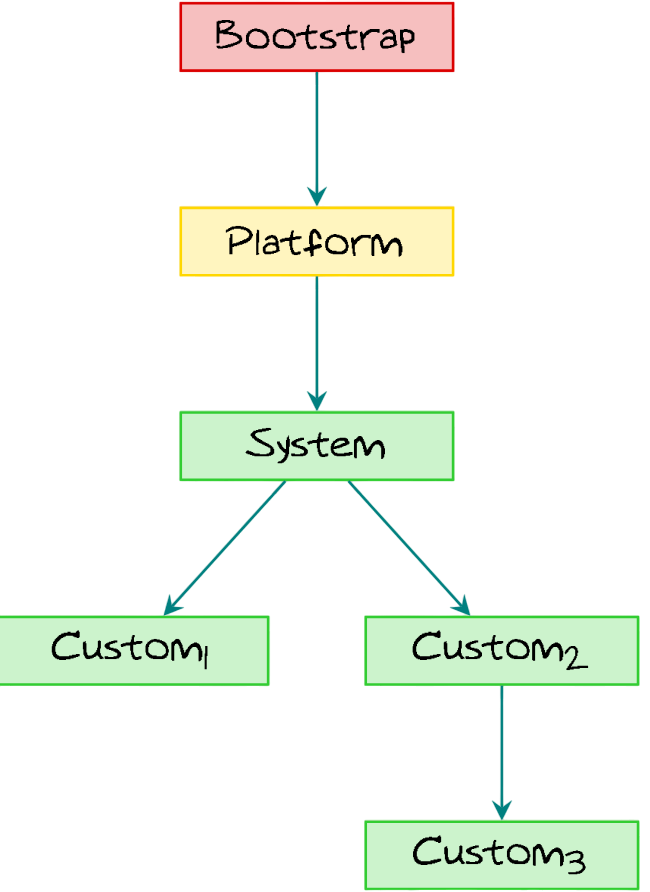
\includegraphics[width=0.45\columnwidth]{img/rij/clHierarchy}
\end{center}

Dall'alto verso il basso:
\begin{itemize}
    \item \textbf{Bootstrap/Primordial/Null Class Loader:} il class loader built-in, scritto in C, non estende \texttt{ClassLoader}; carica le classi Java che fanno parte del core di \texttt{java.base}

    \item \textbf{Platform/Extensions Class Loader:} estende \texttt{Bootstrap}, carica i moduli jdk standard al di fuori di \texttt{java.base}

    \item \textbf{System Class Loader:} Estende \texttt{Platform}, carica classi e jar dal \texttt{CLASSPATH}; può essere customizzato tramite \texttt{-Djava.system.class.loader}
\end{itemize}

%End L5

%Slide pack 08?
%Ricordati di capire meglio cosa sono moduli, packages, CLASSPATH
%Nuova subsection "Modern reflection", Java finisce questa lezione

\subsection{Moduli e Reflection}

Con Java 9 viene introdotta la \textbf{Java Module Platform}, la quale ha gli obiettivi di
\begin{itemize}
    \item Fornire una \textbf{configurazione più affidabile}, mirata a rimpiazzare il meccanismo basato sui classpath a favore di un modo per dichiarare esplicitamente le dipendenze

    \item Una \textbf{più forte encapsulation}, per permettere a ciascun componente di dichiarare quale dei suoi tipi pubblici è accessibile ad altri componenti
\end{itemize}

Un \textbf{modulo} raggruppo classi, interfacce e packages e all'interno di un file \texttt{module-info.java} vengono descritte le dipendenze tra moduli
\begin{minted}{java}
module com.foo.bar {
    requires org.baz.foo;
    exports com.foo.bar.abc;
}
\end{minted}
Questo file viene incluso nel \texttt{jar}.

%Up to s5, esempio
I moduli, per come definiti in questo modo, \textit{bloccano la reflection}, in quanto questa non è in grado di "superare" le restrizioni date dai moduli; è necessario che il modulo "destinazione" apra l'accesso al componente su cui si vuole fare reflection.

Alcune soluzioni:
\begin{itemize}
    \item Aggiungere \texttt{--add-opens} alla JVM per aprire il modulo; ad esempio, per aprire il pacchetto di \texttt{java.lang}, all'interno del modulo \texttt{java.base} verso tutti i moduli senza nome (non dichiarati esplicitamente)
    \begin{minted}{c}
> java --add-opens java.base/java.lang=ALL-UNNAMED ...
    \end{minted}
    Ma non è sempre possibile aggiungere flag alla JVM, come ad esempio usando framework e tool specifici

    \item Aprire il pacchetto/modulo attraverso il relativo file \texttt{module-info.java}, ma anche questo non è detto sia sempre applicabile (e.g., progetti complessi in cui il file non è disponibile)
    \begin{minted}{java}
module com.foo.bar {
    opens com.foo.bar.abc to module.with.reflection;
    requires org.baz.foo;
    exports com.foo.bar.abc;
}
    \end{minted}
    \begin{minted}{java}
module module.with.reflection {
    exports module.with.reflection;
}
    \end{minted}
\end{itemize}

%All'interno di module-info alcuni sono package, altri moduli, buona fortuna per capire quale è quale, hanno lo stesso nome nell'esempio
% Penso che sia: opens package to module, requires module, exports package, ma controlla

%s8
Import e require sono sostanzialmente delle dipendenze, le quali vanno risolte ricorsivamente (ogni modulo ha le proprie dipendenze, ma vanno risolute anche quelle dei moduli chiamati da ogni modulo), possono essere anche cicliche.

Può essere pensato come un grafo di dipendente, la quale chiusura transitiva rappresenta il grafo dei moduli, all'interno della quale ogni arco tra nodi (moduli) rappresenta una dipendenza soddisfatta.

Esiste un tool per vedere questa chiusura: \texttt{jdeps}; un semplice esempio:
\begin{minted}{c}
> jdeps --module-path out --module com.example.app
com.example.app -> java.base
com.example.app -> com.example.utils
\end{minted}
dove \texttt{--module-path} specifica la posizione dei moduli compilati, mentre \texttt{--module} specifica i moduli da analizzare.

Anche \texttt{jshell} deve considerare i moduli: va dato il module path
\begin{minted}{c}
> jshell
    --module-path=<path>
\end{minted}
Assieme agli import
\begin{minted}{c}
    --add-modules=<module>
\end{minted}
E alle open da fare
\begin{minted}{c}
    --add-exports=<module>/<package>:jshell
\end{minted}
Per aprire il package verso la \texttt{jshell}. Al posto di quest'ultimo si può mettere un altro modulo quando usato con \texttt{javac}.

\subsection{Method and Variable Handles}

%s13
La reflection standard è lenta e non sicura, bypassa molti controlli compile-time e dipende da lookup di stringhe.

Vogliamo sostituire questi lookup con \texttt{MethodHandle} e \texttt{VarHandle}, i quali sono più veloci e fortemente tipizzati. Permettono accesso diretto a campi e metodi, preservando i check a compile-time.

Si ha la classe factory di \texttt{MethodHandles}, la quale permette di creare \texttt{MethodHandle}.

Il \texttt{MethodHandles.Lookup} rappresenta i permessi, ovvero determina cosa è accessibile e controlla anche l'accesso ai campi privati (non si usa più il \texttt{setAccessible()}).

L'oggetto \texttt{lookup} può accedere a tutti i membri della classe che lo ha definito, ma non ai membri privati di altre classi. \texttt{MethodHandles.publicLookup} o \texttt{MethodHandles.privateLookupIn} possono restringere o estendere questi permessi.

Gli handle possono effettuare direttamente loro la reificazione
\begin{minted}{java}
VarHandle vh = MethodHandles.lookup()
    .findVarHandle(Employee.class, "surname", String.class);
\end{minted}
oppure trasferirla da un meta-oggetto esistente
\begin{minted}{java}
Field f = Employee.class.getDeclaredField("surname");
f.setAccessible(true);
VarHandle vh = MethodHandles.lookup().unreflectVarHandle(f);
\end{minted}

%Newslides, 09, abbiamo finito con Java
%Il primo parziale arriva fino a qua